
\chapter{Extended PanelOLS Results}
\hrule
\vspace{2em}
Here we display the OFI price impact PanelOLS results for all trading pairs.
\begin{table}[htbp!]
\textbf{BTCUSDT PanelOLS Results for h = 1000ms}
\begin{center}
\begin{tabular}{lclc}
\hline
\textbf{Dep. Variable:}    &         $\Delta p_{\delta}$         & \textbf{  R-squared:         }   &      0.3590      \\
\textbf{Estimator:}        &      PanelOLS      & \textbf{  R-squared (Between):}  &     -0.3865      \\
\textbf{No. Observations:} &      12891080      & \textbf{  R-squared (Within):}   &      0.3590      \\
\textbf{Date:}             &  Tue, Mar 26 2024  & \textbf{  R-squared (Overall):}  &      0.3585      \\
\textbf{Time:}             &      16:15:04      & \textbf{  Log-likelihood     }   &    -6.11e+07     \\
\textbf{Cov. Estimator:}   &     Clustered      & \textbf{                     }   &                  \\
\textbf{}                  &                    & \textbf{  F-statistic:       }   &    7.218e+06     \\
\textbf{Entities:}         &        956         & \textbf{  P-value            }   &      0.0000      \\
\textbf{Avg Obs:}          &     1.348e+04      & \textbf{  Distribution:      }   &  F(1,12890123)   \\
\textbf{Min Obs:}          &       953.00       & \textbf{                     }   &                  \\
\textbf{Max Obs:}          &     1.676e+04      & \textbf{  F-statistic (robust):} &      4743.2      \\
\textbf{}                  &                    & \textbf{  P-value            }   &      0.0000      \\
\textbf{Time periods:}     &       16761        & \textbf{  Distribution:      }   &  F(1,12890123)   \\
\textbf{Avg Obs:}          &       769.11       & \textbf{                     }   &                  \\
\textbf{Min Obs:}          &       1.0000       & \textbf{                     }   &                  \\
\textbf{Max Obs:}          &       956.00       & \textbf{                     }   &                  \\
\textbf{}                  &                    & \textbf{                     }   &                  \\
\hline
\end{tabular}
\begin{tabular}{lcccccc}
             & \textbf{Parameter} & \textbf{Std. Err.} & \textbf{T-stat} & \textbf{P-value} & \textbf{Lower CI} & \textbf{Upper CI}  \\
\hline
\textbf{OFI} &       1.1829       &       0.0172       &      68.871     &      0.0000      &       1.1492      &       1.2166       \\
\hline
\end{tabular}
%\caption{PanelOLS Estimation Summary}
\end{center}
F-test for Poolability: 19.309, \\
Distribution: F(955,12890123),\\
Included effects: Entity.
\end{table}

\begin{figure}[htpb!]
    \centering
    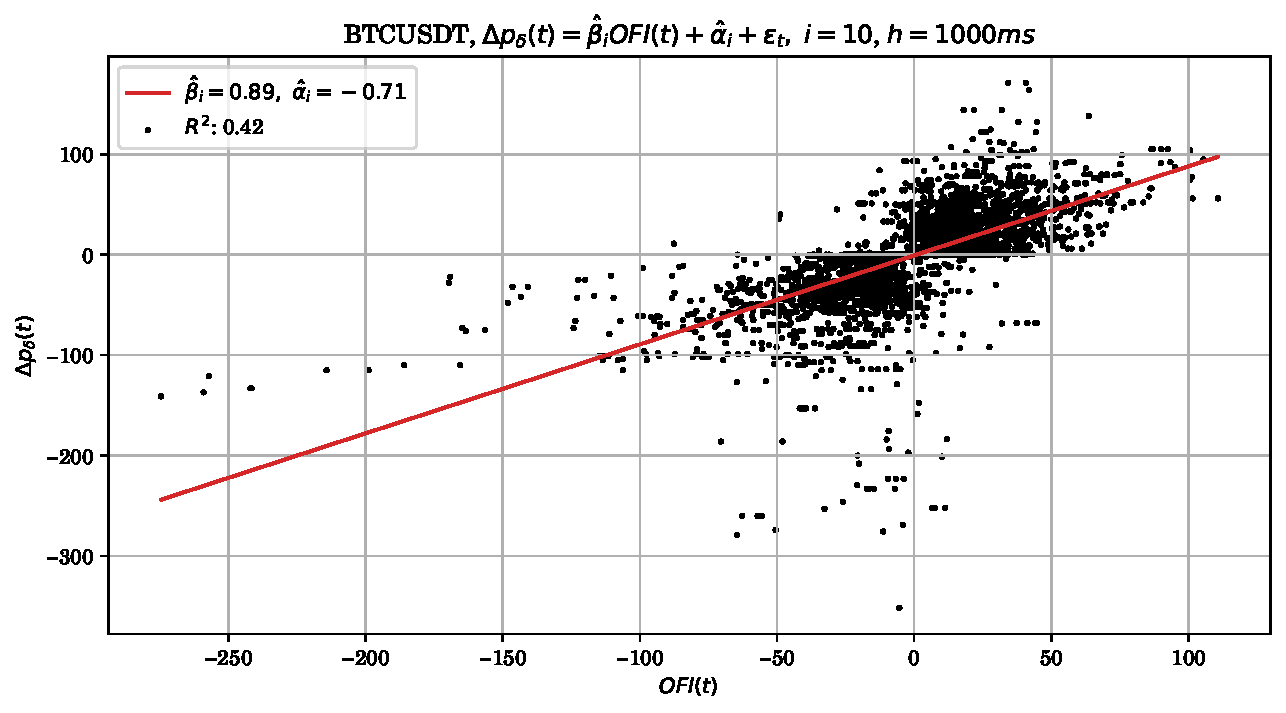
\includegraphics[width=0.8\textwidth]{./images/btcusdt_h=1000ms_contemp_OFI.pdf}
    \caption{OFI contemporaneous regression for an example half-hour window for BTCUSDT.}
\end{figure}

\clearpage




\begin{table*}
\textbf{ETHUSDT PanelOLS Results for h = 1000ms}
\begin{center}
\begin{tabular}{lclc}
\hline
\textbf{Dep. Variable:}    &         $\Delta p_{\delta}$         & \textbf{  R-squared:         }   &      0.3407      \\
\textbf{Estimator:}        &      PanelOLS      & \textbf{  R-squared (Between):}  &     -0.5821      \\
\textbf{No. Observations:} &      13612890      & \textbf{  R-squared (Within):}   &      0.3407      \\
\textbf{Date:}             &  Tue, Mar 26 2024  & \textbf{  R-squared (Overall):}  &      0.3401      \\
\textbf{Time:}             &      16:18:43      & \textbf{  Log-likelihood     }   &    -5.922e+07    \\
\textbf{Cov. Estimator:}   &     Clustered      & \textbf{                     }   &                  \\
\textbf{}                  &                    & \textbf{  F-statistic:       }   &    7.034e+06     \\
\textbf{Entities:}         &        956         & \textbf{  P-value            }   &      0.0000      \\
\textbf{Avg Obs:}          &     1.424e+04      & \textbf{  Distribution:      }   &  F(1,13611933)   \\
\textbf{Min Obs:}          &     1.058e+04      & \textbf{                     }   &                  \\
\textbf{Max Obs:}          &     1.654e+04      & \textbf{  F-statistic (robust):} &      4554.0      \\
\textbf{}                  &                    & \textbf{  P-value            }   &      0.0000      \\
\textbf{Time periods:}     &       16538        & \textbf{  Distribution:      }   &  F(1,13611933)   \\
\textbf{Avg Obs:}          &       823.13       & \textbf{                     }   &                  \\
\textbf{Min Obs:}          &       1.0000       & \textbf{                     }   &                  \\
\textbf{Max Obs:}          &       956.00       & \textbf{                     }   &                  \\
\textbf{}                  &                    & \textbf{                     }   &                  \\
\hline
\end{tabular}
\begin{tabular}{lcccccc}
             & \textbf{Parameter} & \textbf{Std. Err.} & \textbf{T-stat} & \textbf{P-value} & \textbf{Lower CI} & \textbf{Upper CI}  \\
\hline
\textbf{OFI} &       0.0891       &       0.0013       &      67.483     &      0.0000      &       0.0866      &       0.0917       \\
\hline
\end{tabular}
%\caption{PanelOLS Estimation Summary}
\end{center}
F-test for Poolability: 21.726, \\
Distribution: F(955,13611933), \\
Included effects: Entity.
\end{table*}

\begin{figure*}[htpb]
    \centering
    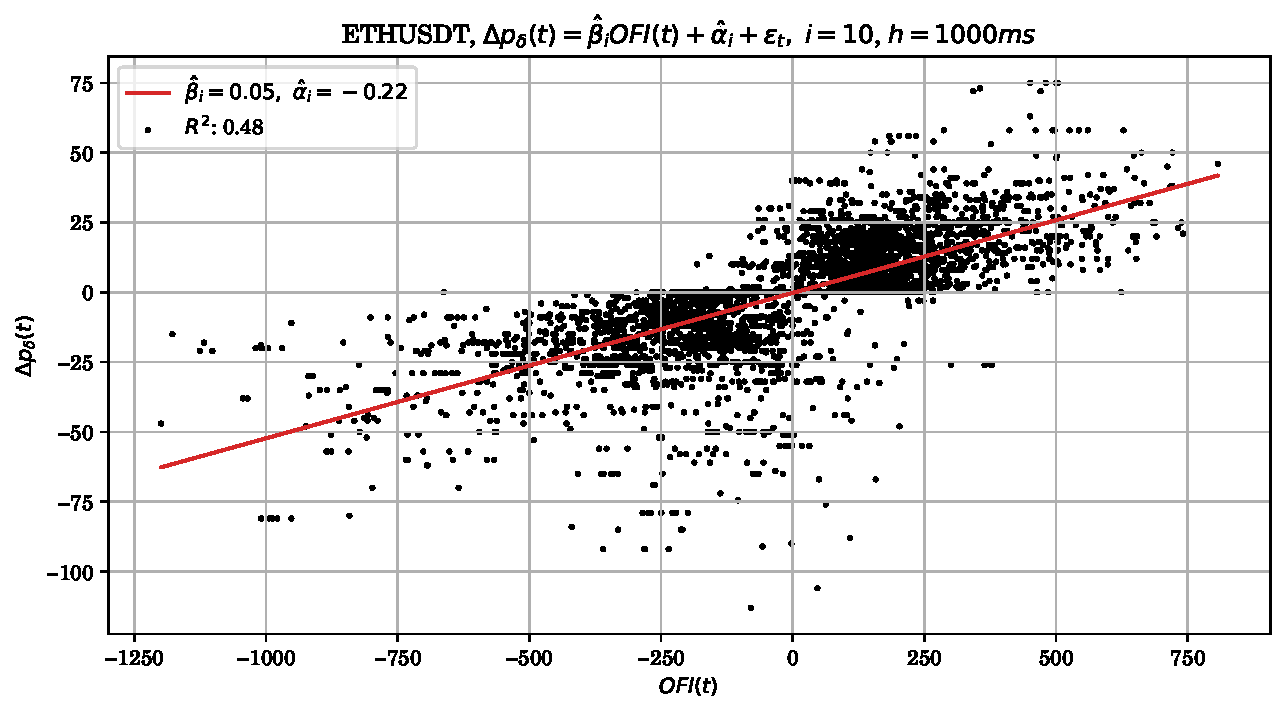
\includegraphics[width=0.8\textwidth]{./images/ethusdt_h=1000ms_contemp_OFI.pdf}
    \caption{OFI contemporaneous regression for an example half-hour window for ETHUSDT.}
\end{figure*}
\clearpage




\begin{table*}
\textbf{SOLUSDT PanelOLS Results for h = 1000ms}
\begin{center}
\begin{tabular}{lclc}
\hline
\textbf{Dep. Variable:}    &         $\Delta p_{\delta}$         & \textbf{  R-squared:         }   &      0.2828      \\
\textbf{Estimator:}        &      PanelOLS      & \textbf{  R-squared (Between):}  &     -0.3992      \\
\textbf{No. Observations:} &      13334051      & \textbf{  R-squared (Within):}   &      0.2828      \\
\textbf{Date:}             &  Tue, Mar 26 2024  & \textbf{  R-squared (Overall):}  &      0.2824      \\
\textbf{Time:}             &      16:21:12      & \textbf{  Log-likelihood     }   &    -5.176e+07    \\
\textbf{Cov. Estimator:}   &     Clustered      & \textbf{                     }   &                  \\
\textbf{}                  &                    & \textbf{  F-statistic:       }   &    5.258e+06     \\
\textbf{Entities:}         &        957         & \textbf{  P-value            }   &      0.0000      \\
\textbf{Avg Obs:}          &     1.393e+04      & \textbf{  Distribution:      }   &  F(1,13333093)   \\
\textbf{Min Obs:}          &       7478.0       & \textbf{                     }   &                  \\
\textbf{Max Obs:}          &     1.647e+04      & \textbf{  F-statistic (robust):} &      428.29      \\
\textbf{}                  &                    & \textbf{  P-value            }   &      0.0000      \\
\textbf{Time periods:}     &       16473        & \textbf{  Distribution:      }   &  F(1,13333093)   \\
\textbf{Avg Obs:}          &       809.45       & \textbf{                     }   &                  \\
\textbf{Min Obs:}          &       1.0000       & \textbf{                     }   &                  \\
\textbf{Max Obs:}          &       957.00       & \textbf{                     }   &                  \\
\textbf{}                  &                    & \textbf{                     }   &                  \\
\hline
\end{tabular}
\begin{tabular}{lcccccc}
             & \textbf{Parameter} & \textbf{Std. Err.} & \textbf{T-stat} & \textbf{P-value} & \textbf{Lower CI} & \textbf{Upper CI}  \\
\hline
\textbf{OFI} &       0.0128       &       0.0006       &      20.695     &      0.0000      &       0.0116      &       0.0140       \\
\hline
\end{tabular}
%\caption{PanelOLS Estimation Summary}
\end{center}
F-test for Poolability: 15.871, \\
Distribution: F(956,13333093), \\
Included effects: Entity.
\end{table*}

\begin{figure*}[htpb]
    \centering
    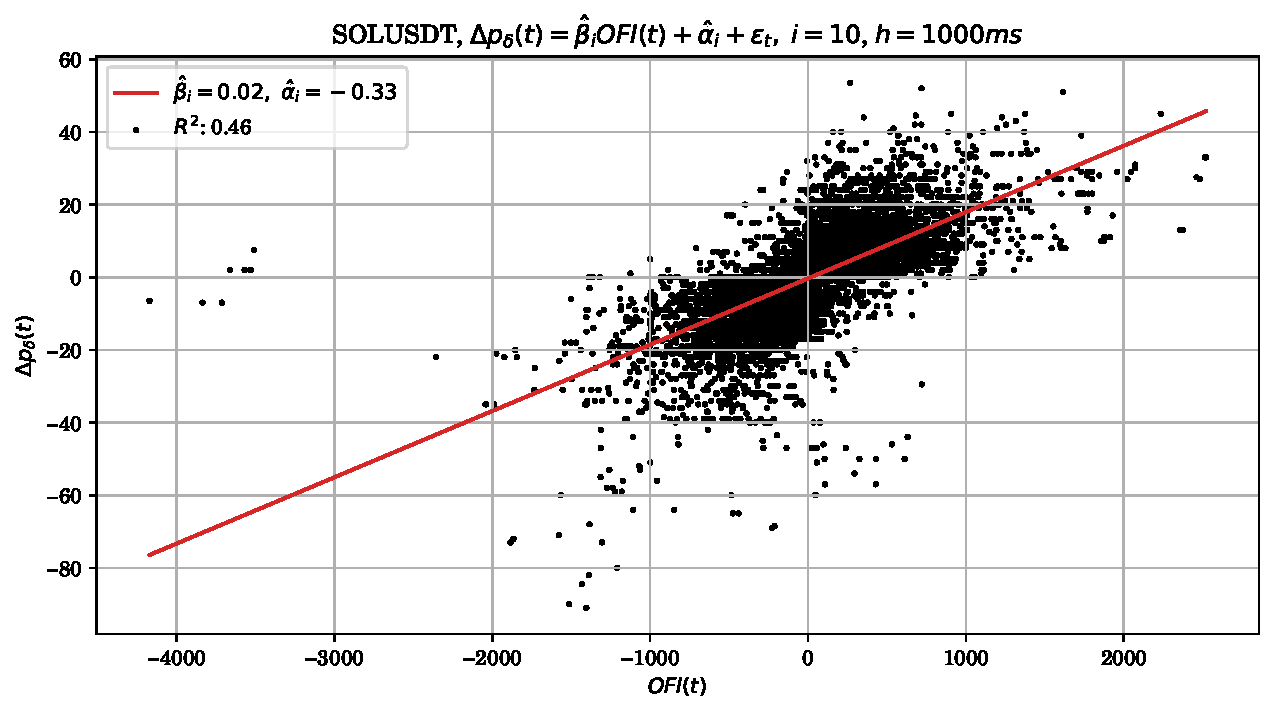
\includegraphics[width=0.8\textwidth]{./images/solusdt_h=1000ms_contemp_OFI.pdf}
    \caption{OFI contemporaneous regression for an example half-hour window for SOLUSDT.}
\end{figure*}

\clearpage




\begin{table*}
\textbf{MATICUSDT PanelOLS Results for h = 1000ms}
\begin{center}
\begin{tabular}{lclc}
\hline
\textbf{Dep. Variable:}    &         $\Delta p_{\delta}$         & \textbf{  R-squared:         }   &      0.4133      \\
\textbf{Estimator:}        &      PanelOLS      & \textbf{  R-squared (Between):}  &     -0.0188      \\
\textbf{No. Observations:} &      11294487      & \textbf{  R-squared (Within):}   &      0.4133      \\
\textbf{Date:}             &  Tue, Mar 26 2024  & \textbf{  R-squared (Overall):}  &      0.4130      \\
\textbf{Time:}             &      16:23:26      & \textbf{  Log-likelihood     }   &    -1.58e+07     \\
\textbf{Cov. Estimator:}   &     Clustered      & \textbf{                     }   &                  \\
\textbf{}                  &                    & \textbf{  F-statistic:       }   &    7.955e+06     \\
\textbf{Entities:}         &        956         & \textbf{  P-value            }   &      0.0000      \\
\textbf{Avg Obs:}          &     1.181e+04      & \textbf{  Distribution:      }   &  F(1,11293530)   \\
\textbf{Min Obs:}          &       5754.0       & \textbf{                     }   &                  \\
\textbf{Max Obs:}          &     1.639e+04      & \textbf{  F-statistic (robust):} &      2882.6      \\
\textbf{}                  &                    & \textbf{  P-value            }   &      0.0000      \\
\textbf{Time periods:}     &       16388        & \textbf{  Distribution:      }   &  F(1,11293530)   \\
\textbf{Avg Obs:}          &       689.19       & \textbf{                     }   &                  \\
\textbf{Min Obs:}          &       1.0000       & \textbf{                     }   &                  \\
\textbf{Max Obs:}          &       956.00       & \textbf{                     }   &                  \\
\textbf{}                  &                    & \textbf{                     }   &                  \\
\hline
\end{tabular}
\begin{tabular}{lcccccc}
             & \textbf{Parameter} & \textbf{Std. Err.} & \textbf{T-stat} & \textbf{P-value} & \textbf{Lower CI} & \textbf{Upper CI}  \\
\hline
\textbf{OFI} &     3.108e-05      &     5.789e-07      &      53.690     &      0.0000      &     2.995e-05     &     3.222e-05      \\
\hline
\end{tabular}
%\caption{PanelOLS Estimation Summary}
\end{center}
F-test for Poolability: 15.992, \\
Distribution: F(955,11293530), \\
Included effects: Entity.
\end{table*}

\begin{figure*}[htpb]
    \centering
    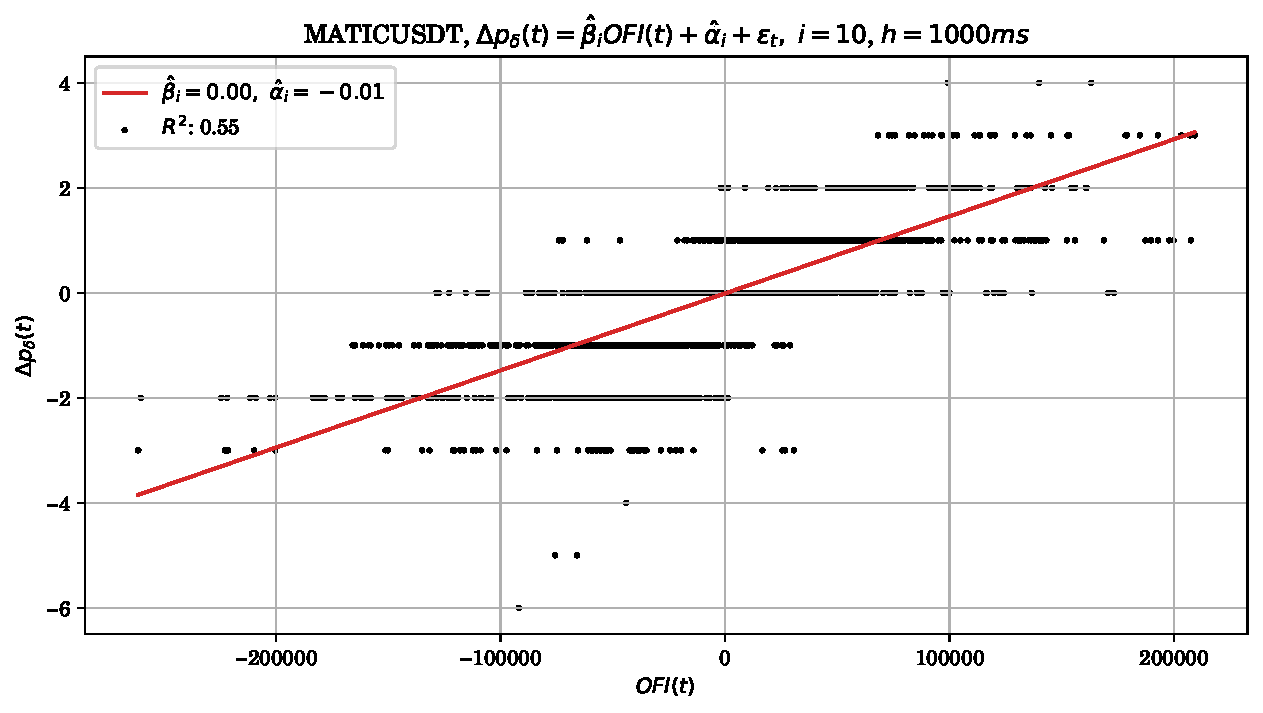
\includegraphics[width=0.8\textwidth]{./images/maticusdt_h=1000ms_contemp_OFI.pdf}
    \caption{OFI contemporaneous regression for an example half-hour window for MATICUSDT.}
    \label{fig:contemp_OFI_maticusdt}
\end{figure*}

